\section{Approximation algorithms}

\subsection{Disposition}

\begin{enumerate}
 \item \textbf{Def. P, NP, NP-hard \& NPC}
    \subitem  Tegn og MEGET hurtig def.
 \item \textbf{Løsning af NPC problemer}
    \subitem Direkte løsning (exp time)
    \subitem Heuristics (ingen garantier)
    \subitem Approximation Algoritmer (garanteret kvalitet og runtime bounds)
 \item \textbf{Def. Approximationalgoritmer}
    \subitem Minimization ($\frac{C}{C^*} \leq \rho$)
    \subitem Maximization ($\frac{C^*}{C} \leq \rho$)
 \item \textbf{Def. Approximation Schemes}
    \subitem PTAS \& FPTAS
 \item \textbf{Def. Algoritmedesign}
    \subitem Relaxation (for at få lower bound)
    \subitem Ændre relaxed version til feasible solution
 \item \textbf{Relaxation af TSP}
    \subitem Kigger kun på Metric TSP
    \subitem Relax til minimum spanning tree
    \subitem Bevis theorem 35.2 (APPROX-TSP-TOUR(G,c) har approx. ratio $2$)
 \item \textbf{Approximering af general TSP}
    \subitem Approximering af generel TSP $\in$ NP-hard
    \subitem Bevis. (vha. gap creating reduction)
\end{enumerate}

\subsection{Emne detaljer}

Følgende afsnit indeholder detaljer om hvert punkt i dispositionen ovenfor (og muligvis flere ting også).

\subsubsection{Def. P, NP, NP-hard \& NPC}

Lad os starte med lige at kigge på de kompleksitetsklasser vi har arbejdet med her i kurset.
\begin{center}
 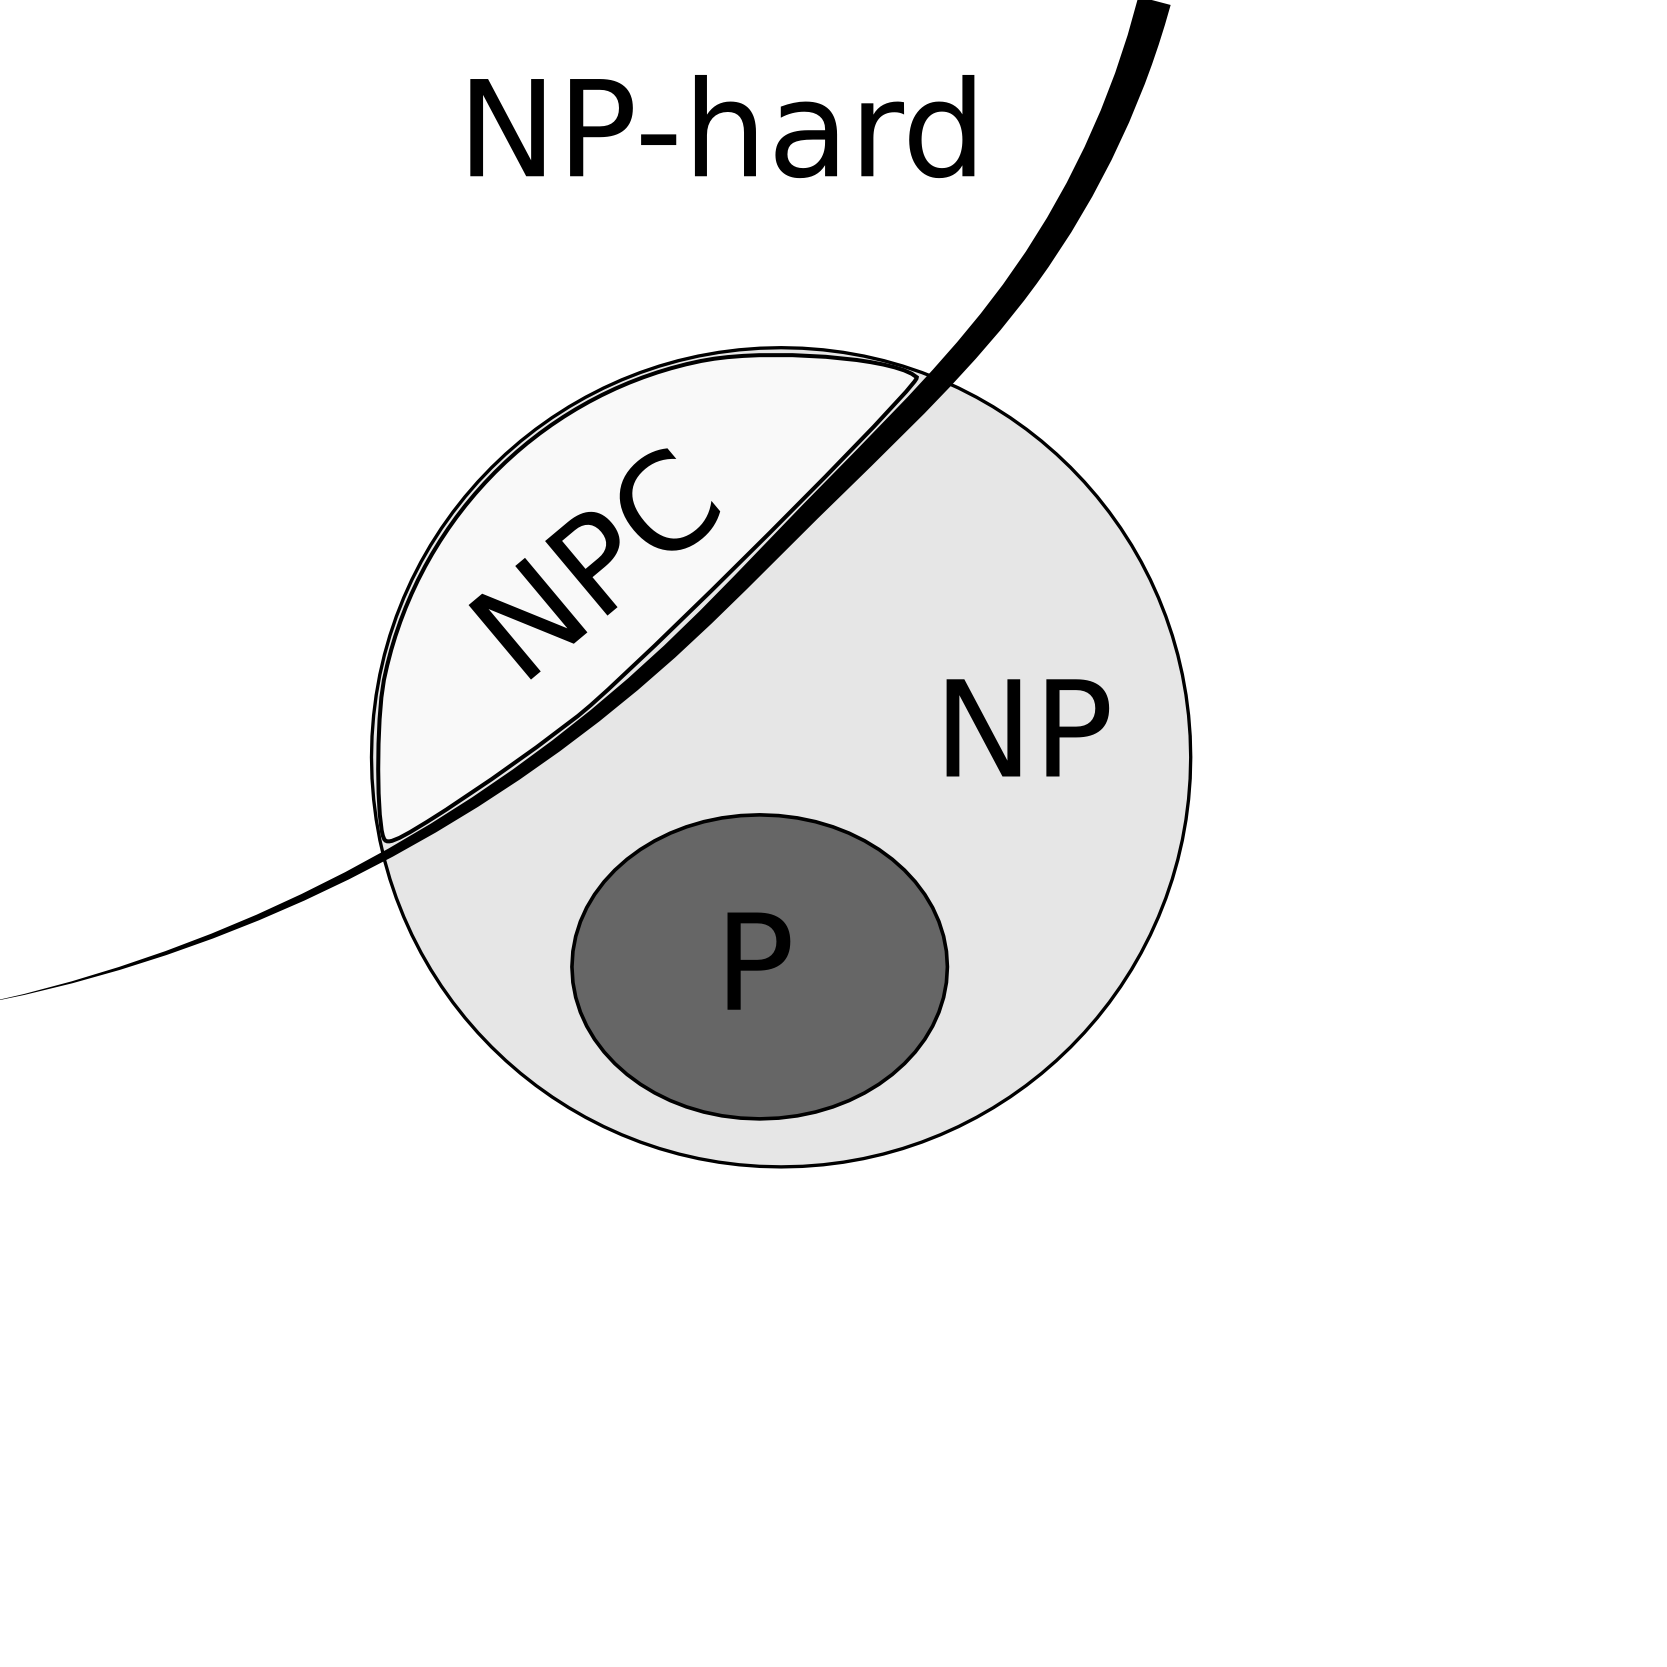
\includegraphics[bb=0 0 400 400,scale=0.3]{./PNPNPC.png}
 % PNPNPC.png: 1667x1667 pixel, 300dpi, 14.11x14.11 cm, bb=0 0 400 400
\end{center}


\paragraph{P}
~\\
~\\
Kompleksitetsklassen $P$ er formelt defineret således:
\begin{align*}
 P = \left\lbrace L \subseteq \left\lbrace 0,1 \right\rbrace^* | \exists \text{ TM } M_L \text{ der afgører L i polynomiel tid } \right\rbrace
\end{align*}
Altså klassen af beslutningsproblemer der kan blive bestemt af en deterministisk Turing Maskine hvor antallet af ``steps'' maskinen udfører for et givent $x$ maksimalt er $\rho(x)$ for et givent polynomiel $\rho$.\\
 
Intuivit ser vi kompleksitetsklassen $P$ som en klasse for problemer for hvilket vi kender en effektiv løsning. Altså ethvert problem med worst-case kørselstid på formen $O(n^k)$ for et givent $k$.

At worst-case kørseltid på et problem er polynomiel betyder dog ikke reelt at det er et nemt problem (modsat hvad Cobham's Thesis påstår). I hele den analyse ignorerer vi fuldkommen konstanter, samt forventet kørselstid som I mange tilfælde kan få ``sværere'' problemer til at køre bedre end ``nemme'' problemer i $P$.


\paragraph{NP}
~\\
~\\
Kompleksitetsklassen $NP$ er lidt mere kluntet formelt defineret, så vi starter lige med intuitionen først.

Intuitivt kan $NP$ ses som klassen af beslutningsproblemer for hvilket ``yes'' instanserne kan verificeres i polynomiel tid på en deterministisk Turing Maskine. Altså er det komplekse problemer med eksponentiel løbetid, men hvor løsningen til et sådant problem nemt kan verificeres til at være korrekt.\\
~\\
Kompleksitetsklassen $NP$ er formelt defineret således:
\begin{align*}
 NP = \left\lbrace L \subseteq \left\lbrace 0,1 \right\rbrace^* | \exists \rho \in Z[x], L' \in P, \forall x \in \left\lbrace 0,1 \right\rbrace^* : ( x \in L \Leftrightarrow \exists y \in \left\lbrace 0,1 \right\rbrace^* : |y| \leq \rho(|x|) \wedge \left\langle x,y \right\rangle \in L') \right\rbrace
\end{align*}
Definitionen skal forståes således: Vi har et sprog $L' \in P$, samt et polynomiel $\rho$. Vi tænker så nu på et sæt af binære strenge af længde maksimalt $\rho(|x|)$, hvor disse representerer mulige løsninger til probleminstansen $x$. Med denne fortolkning bliver $\left\langle x,y \right\rangle \in L'$ så måden hvorpå vi tester om en given løsning $y$ virkelig er en korrekt løsning. 

Denne form for søgningsproblem kaldes ofte for et simpelt søgningsproblem, da den kan verificeres i polynomiel tid, men ikke løses deri (antaget $P \neq NP$).\\

For at løse et givent NP problem kunne vi så løbe igennem alle mulige løsninger for $y$, som sammenlagt ville være $2^{\rho(|x|)+1}-1$, og for hver af dem tjekke $\left\langle x,y \right\rangle \in L'$. Det ønsker vi dog ikke, da det ville tage eksponentiel tid. I stedet forsøger man ofte at finde snedige måder at lave speed-ups og/eller lave approximationsalgoritmer af forskellige art.

Og i visse tilfælde er man også heldig at finde en algoritme i $P$ for et $NP$ problem, hvorved man har vist at problemet i virkeligheden ligger i $P$ som jo er et subset af $NP$.

\paragraph{NP-hard}
~\\
~\\
Et sprog defineres som NP-hard såfremt der gælder:

\begin{align*}
 \forall L' \in NP: L' \leq L
\end{align*}

Altså gælder der, at ethvert sprog $L'$ i NP kan reduceres til $L$. Intuitionen er her, at algoritmen til at løse NP-hard problemet er så stærk (eller generel) at den kan bruges til at løse ethvert andet problem i NP. Man siger desuden, at et NP-hard problem således er mindre sandsynlig end noget andet sprog i NP, til at være i P.\\

Navnet kan dog være lidt forvirrende, da et NP-hard problem faktisk ikke behøver være i NP og hvis de er, så kaldes de faktisk ikke engang bare NP-hard længere.

\paragraph{NPC}
~\\
~\\
NP-Complete (NPC) er den særlige klasse af problemer der både er NP-hard og befinder sig i NP. Formelt defineret således: 

\begin{align*}
 NPC = \left\lbrace L \in \left\lbrace 0,1 \right\rbrace^* | L \in NP \wedge (\forall L' \in NP: L' \leq L) \right\rbrace
\end{align*}

NPC problemer er særligt interessante, da vi kan bruge dem til at bevise et givent problem er NP-Complete, således vi ikke spilder tid på forsøg med at finde en algoritme i $P$ for problemet (antaget $P\neq NP$). Dette gør vi vha. noget vi kalder reduktioner.


\subsubsection{Løsning af NPC problemer}

Men hvad så hvis vi har et givent NPC problem og vi egentlig gerne vil løse det og ikke bare bruge det til at vise andre problemer er i NPC? Så har vi grundlæggende 3 muligheder vi kan benytte os af:

\begin{description}
 \item[Direkte løsning:] Hvis vi har et meget lille input, så kan det måske være fint at bruge algoritmen direkte og så leve med den eksponentielle kørselstid. En sådan algoritme vil dog ofte i praksis være fuldkommen umulig at udregne direkte i ens levetid, selv for rimelig små input. Der er dog også tilfælde hvor algoritmer med worst-case eksponentiel kørselstid har langt bedre kørselstid i praksis, hvorfor direkte exact løsning er fint.
 \item[Isoler special cases:] Flere NPC problemer har special cases der kan løses i polynomiel tid. Man kunne bruge det problem i stede såfremt den specifikke special case løser ens problem.
 \item[Approximation \& Heuristics:] Hvis de to ovenstående løsninger ikke er mulige, så kan man i stedet forsøge at finde ``nær-optimale'' løsninger i polynomiel tid vha. approximationsalgoritmer eller heuristikker.
\end{description}

Vi vil i dette emne fokusere på såkaldte approximationsalgoritmer.


\subsubsection{Approximationsalgoritmer}

En polynomieltids approximationsalgoritme er en algoritme der for et givent optimeringsproblem returnerer ``nær-optimale'' løsninger i polynomiel tid (enten forventet eller worst-case).\\

Lad os forestille os vi har et givent optimeringsproblem hvori hver given løsning har en associteret ``cost'' og vi ønsker at finde en nær-optimal løsning til dette problem. Afhængig af problemet ønsker vi så at finde løsninger der maksimerer eller minimerer cost, i.e. enten et maksimeringsproblem eller minimeringsproblem.

Vi siger så, at en given algoritme for dette problem har en approximations ratio $\rho(n)$ hvis, for ethvert input af størrelsen $n$, cost $C$ af den producerede løsning er inden for en faktor $\rho(n)$ af en cost $C^*$ for en optimal løsning. Altså:
\begin{align*}
 \max(\frac{C}{C^*},\frac{C^*}{C}) \leq \rho(n)
\end{align*}
Eller sagt på en anden måde, for et givent minimeringsproblem (hvor $0 < C^* \leq C$):
\begin{align*}
 \frac{C}{C^*} \leq \rho(n)
\end{align*}
Og for et givent maksimeringsproblem (hvor $0 < C \leq C^*$):
\begin{align*}
 \frac{C^*}{C} \leq \rho(n)
\end{align*}
~\\
Vi kalder en algoritme der opnår en approximerings ratio på $\rho(n)$ for en $\rho(n)$-approximationsalgoritme. Derved er en 1-approximationsalgortime ækvivalent med en optimal løsning.

\subsubsection{Approximation Schemes}

Nogle NP-Complete problemer har den egenskab, at de kan tillade polynomieltids approximationsalgoritmer der opnår gradvist mindre approximations ratios ved at bruge mere beregningstid. Altså at man derved kan lave en trade-off mellem beregningstid og kvaliteten af approximationen. En sådan mekanisme hedder et approximations scheme!\\

Et approximations scheme for et optimeringsproblem er en approximationsalgoritme der som input ikke blot tager en given probleminstans, men som også tager en værdi $\varepsilon > 0$ således, at for ethvert fast $\varepsilon$, så er schemet en $(1+\varepsilon)$-approximationsalgoritme.

\paragraph{PTAS}
~\\
~\\

Vi siger således, at et approximations scheme er et polynomieltids approximations scheme, forkortet PTAS, hvis for ethvert fast $\varepsilon > 0$, schemet kører i polynomiel tid i størrelsen $n$ af dets input probleminstans.

\paragraph{FPTAS}
~\\
~\\

Vi siger desuden, at et approximations scheme er et fuldt polynomieltids approximations scheme, hvis det er et approximations scheme og dets kørselstid er polynomiel både i $1/\varepsilon$ og i størrelsen $n$ af dets input probleminstans.

F.eks. kunne et sådant scheme have kørselstid $O((1/\varepsilon)^2 n^3)$. Med sådan et scheme ville enhver nedadgående konstant-faktor regulering af $\varepsilon$ kunne opnås ved en tilsvarende opadgående konstant-faktor regulering af kørselstiden.

\subsubsection{Algoritmedesign}

Men hvordan designer man så en approximationsalgoritme? Og hvordan sammenligner man den med den optimale, når nu man oftest ikke ved hvad den optimale løsning er?\\

Ideen er simpelthen den, at fremfor at forsøge sammenligning og approximation på problemet direkte, så laver man ofte en approximationsalgoritme ved at konstruere en ``relaxation'' af det givne problem, hvorved man også kan få et lower/upper bound (afhængig af om vi taler om minimization eller maximization) ud fra denne relaxation og så til sidst ændrer man ens relaxed version tilbage til en mulig løsning for problemet, uden at ofre algoritmekørselstiden i nogen særlig grad.\\

Lad os nu kigge på et eksempel på en sådan relaxation. I dette tilfælde en relaxation af TSP.

\subsubsection{Relaxation af TSP}

I Traveling salesman problemet, eller TSP, er vi givet en komplet urettet graf $G=(V,E)$ med en ikke-negativ cost $c(u,v)$ for hver kant $(u,v) \in E$. Vi må nu finde en hamilton cycle (en tour der går igennem alle knuder) i G, hvor denne minimerer samlet cost. Som en udvidelse på notationen, lad $c(A)$ betyde den totale cost af alle kanter i et subset $A \subseteq E$, altså:
\begin{align*}
 c(A) = \sum_{(u,v) \in A} c(u,v)
\end{align*}

\paragraph{Metric TSP}
~\\
~\\
En special case har vi så i metric TSP hvor cost funktionen tilfredsstiller den såkaldte trekantsulighed. Trekantsuligheden sikrer at, man populært sagt ikke kan lave genveje, således at en direkte vej fra by $u$ til by $w$ aldrig er længere end en omvej via. en tredje by $v$. Eller skrevet lidt mere formelt op:
\begin{align*}
 c(u,w) \leq c(u,v) + c(v,w)
\end{align*}
~\\
Medmindre andet nævnes i gennemgangen herefter, så vil vi som udgangspunkt antage at vi har instanser af metric TSP (således trekantsuligheden gælder), og laver desuden den yderligere begrænsning kun at kigge på symmetriske varianter af TSP, således $c(u,w) = c(w,u)$.\\
~\\

\paragraph{Relaxation til minimum spanning tree}
~\\
~\\
For at få en ide om hvad approximationsalgoritmer har at byde på, så vil vi nu kigge på en approximationsalgoritme for metric TSP. Så vi skal starte med at finde en passende relaxation der giver os mulighed for at lave ordentlig optimering, samt giver os et lower bound på den optimale løsning.

En sådan struktur får vi i form af et minimum spanning tree, da vægten af et sådan træ er et lower bound på længden af den optimale TSP tour. Dette kan ses ved, at en given optimal tur hvor vi sletter en kant, øjeblikkeligt bliver til et spanning tree.

Vi bruger altså et minimum spanning tree til at konstruere en tour der er intet mere end 2 gange vægten af træet, igen antaget metric TSP.
Følgende algoritme gør netop dette, ved at konstruere minimum spanning træet vha. MST-PRIM algoritmen der kaldes som subrutine.
\begin{center}
 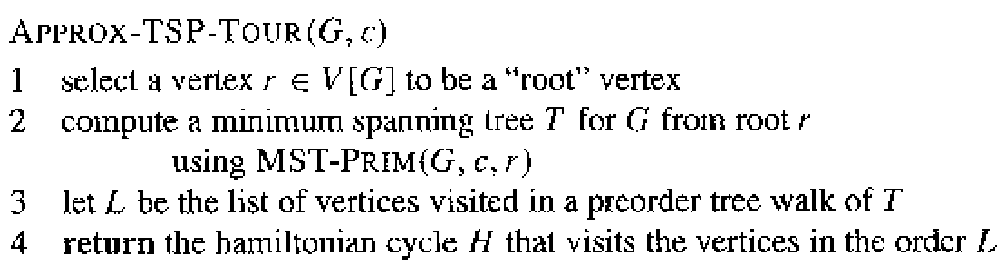
\includegraphics[bb=0 0 754 196,scale=0.5]{./approxTSPTour.png}
 % approxTSPTour.png: 1005x261 pixel, 96dpi, 26.59x6.90 cm, bb=0 0 754 196
\end{center}
Altså har vi en algoritme der gør følgende:
\begin{enumerate}
 \item Vælger en given knude $r$ til at være roden.
 \item Konstruer et minimum spanning tree $T$ fra roden $r$ på hele grafen $G$
 \item Lav et pre-order walk i $T$ og opbyg en liste $L$ af knuder set på denne rute. (OBS: et pre-order walk tilføjer knuder rekursivt til listen hver gang den ser dem, også selvom de har børn)
 \item Lav en Hamilton Cycle $H$ der følger knuderne som listet i $L$, ignorerende duplikater.
 \item Denne Hamilton Cycle er så vores returnede tourløsning $H$
\end{enumerate}

Kørslen af denne algoritme er illustreret herunder:
\begin{center}
 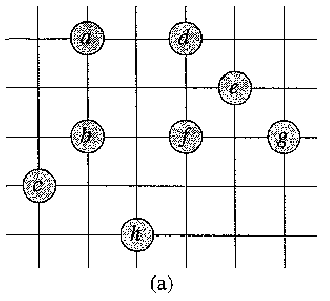
\includegraphics[bb=0 0 247 226,scale=0.7]{./approxTSP1.png}
 % approxTSP1.png: 330x301 pixel, 96dpi, 8.73x7.96 cm, bb=0 0 247 226
 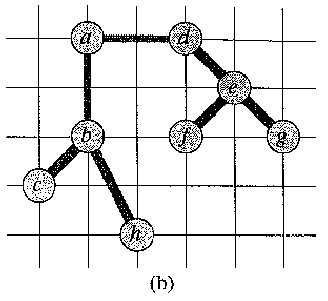
\includegraphics[bb=0 0 247 226,scale=0.7]{./approxTSP2.png}
 % approxTSP1.png: 330x301 pixel, 96dpi, 8.73x7.96 cm, bb=0 0 247 226
 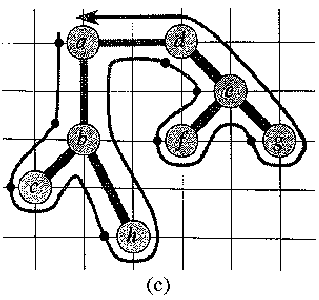
\includegraphics[bb=0 0 247 226,scale=0.7]{./approxTSP3.png}
 % approxTSP1.png: 330x301 pixel, 96dpi, 8.73x7.96 cm, bb=0 0 247 226
 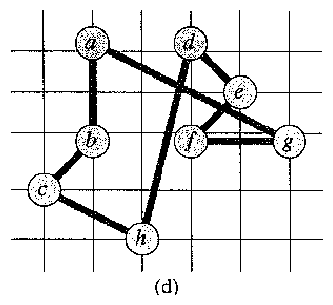
\includegraphics[bb=0 0 247 226,scale=0.7]{./approxTSP4.png}
 % approxTSP1.png: 330x301 pixel, 96dpi, 8.73x7.96 cm, bb=0 0 247 226
\end{center}
Vi har altså ovenstående endelige tour $H$, med en samlet cost på $19.074$ (vides fra teksten). Den optimale tour $H^*$ for samme graf er dog den følgende, som har en samlet cost på kun $14.715$. Altså en godt $23\%$ bedre tour:

\begin{center}
  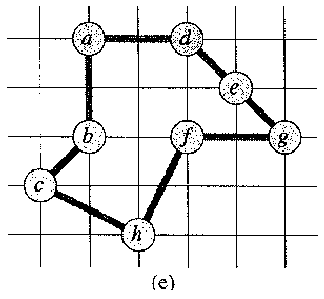
\includegraphics[bb=0 0 247 226,scale=0.7]{./approxTSPOpt.png}
 % approxTSP1.png: 330x301 pixel, 96dpi, 8.73x7.96 cm, bb=0 0 247 226
\end{center}

Ovenstående algoritme har en kørselstid på $\Theta(V^2)$ og vi vil nu bevise, at det den approximerer metric TSP så godt, at den altid returnere en tour der maksimalt er 2 gange så dyr som den optimale tour.\\
~\\
\textbf{Theorem 35.2:} APPROX-TSP-TOUR er en polynomiel 2-approximationsalgoritme for metric special casen af traveling salesman problemet

\begin{proof}
 Vi ved allerede at APPROX-TSP-TOUR har en polynomiel kørselstid, så det behøver vi ikke vise. 

Så lad nu $H^*$ være den optimale tour for et givent sæt knuder. Siden vi, som tidligere omtalt, kan opnå et spanning tree ved blot at fjerne en kant fra turen, så ved vi, at vægten af minimum spanning træet $T$ er et lower bound på cost af den optimale tur således:
\begin{align*}
 c(T) \leq c(H^*)
\end{align*}
Et fuldt pre-order walk af $T$ lister så de knuder der først er blevet besøgt og også alle gange de er set igen fordi de havde børn man besøgte i et undertræ. Denne walk kan vi kalde $W$ og, for vores eksempel indeholdte den:
\begin{center}
 \textit{a, b, c, b, h, b, a, d, e, f, e, g, e, d, a}
\end{center}
Siden et fuldt walk traverserer hver kant i $T$ præcis 2 gange, så har vi:
\begin{align*}
 c(W) = 2c(T)
\end{align*}
Sammensætter vi de to costudtryk vi nu har kigget på, så får vi at:
\begin{align*}
 c(W) \leq 2c(H^*)
\end{align*}
Så costen relateret til $W$ er inden for en faktor 2 af den optimale tour. $W$ er dog ikke en tour, da den besøger visse knuder mere end en gang, hvorfor vi også i algoritmen ignorerer duplikater ved opbygning af en Hamilton Cycle $H$. Dette kan vi gøre, da trekantsuligheden gælder og vi derfor ved det ikke forøger vores cost at slette en knude fra listen $W$. Knuderne omkring denne i listen bliver blot koblet i stedet (i.e. hvis $v$ var imellem $w$ og $u$, og $v$ slettes, så går turen direkte fra $w$ til $u$). 

Så efter at have fjernet alle med undtagelse af første visit til en knude får vi følgende liste, som så er vores Hamilton Cycle $H$:
\begin{center}
 \textit{a, b, c, h, d, e, f, g}
\end{center}
Siden denne $H$ blev skabt ved at fjerne knuder fra $W$, så har vi:
\begin{align*}
 c(H) \leq c(W)
\end{align*}
Samler vi nu udtrykkene for cost af $W$ i forhold til den optimale løsning og resultatet ovenfor, så får vi:
\begin{align*}
 c(H) \leq 2c(H^*)
\end{align*}
Altså har vi nu bevist, at APPROX-TSP-TOUR er en 2-approximationsalgoritme for metric TSP.
\end{proof}

\subsubsection{Approximering af general TSP}

Hvis vi nu ikke havde antaget vores TSP instans var en metric TSP instans, så havde vi dog haft et problem, da det er bevisligt at generel TSP ikke har nogen polynomieltids approximationsalgoritme medmindre $P \neq NP$. Det vil vi nu bevise.\\
~\\
\textbf{Theorem 35.3:} Hvis $P \neq NP$, så for enhver konstant $\rho \geq 1$, eksisterer der ingen polynomieltids approximationsalgoritme med approximationsratio $\rho$ for generel TSP. Det siges derfor, at approximation af generel TSP er NP-hard.

\begin{proof}
 Vi vil bevise dette theorem ved at konstruere en såkaldt ``gap creation reduction'' fra Hamilton Cycle. Det bliver således et proof-by-contradiction.

Lad os forestille os, modsat bedre vidende, at der rent faktisk eksisterede en polynomieltids approximationsalgoritme $A$ med approximationsratio $\rho$ for $\rho \geq 1$. Uden tab af generalitet antager vi, at $\rho$ er et heltal (evt. ved at runde op hvis nødvendigt). Vi vil så vise hvorledes man kan bruge $A$ til at løse instanser af Hamilton Cycle problemet i polynomiel tid. Siden Hamilton Cycle problemet er NP-Complete, så vil en polynomieltids løsning til problemet betyde $P = NP$.\\

Lad $G=(V,E)$ være en instans af Hamilton Cycle problemet. We ønsker nu at tjekke effektivt hvorvidt $G$ indeholder en hamilton cycle vha. vores antagede approximationsalgoritme $A$. Vi laver derfor en alternativ reduktion Hamilton Cycle $\leq$ TSP, ved at lave $G$ om til en instans af $TSP$ således:\\

Lad $G'=(V,E')$ være den komplette graf hvor $E'$ er alle tænkelige kanter imellem knuder, altså:
\begin{align*}
 E' = \left\lbrace (u,v) : u,v \in V \text{ and } u \neq v \right\rbrace
\end{align*}
Tillæg en heltals cost på hver kant i $E'$ således:
\begin{itemize}
 \item Hvis $(u,v) \in E$: $c(u,v) = 1$
 \item Ellers: $\rho|V|+1$
\end{itemize}
Denne graf og costfunktion kan konstrueres i polynomiel tid i længden af $V$ og $E$, så det er en polynomieltids reduktion.

Hvis vi nu kigger på det resulterede TSP problem $(G',c)$, så hvis den originale graf $G$ havde en hamilton cycle $H$, så har cost funktionen $c$ givet hver kant i $H$ cost 1 og derved har $(G',c)$ en tour med cost $|V|$. På den anden side, hvis $G$ ikke indeholdte en hamilton cycle, så må enhver tour i $G'$ bruge en kant der ikke er i $E$. Men enhver tour der bruger en sådan kant må have cost mindst:
\begin{align*}
 (\rho|V|+1)+(|V|-1) &= \rho|V| + |V| \\
		     &> \rho|V|
\end{align*}
Fordi kanterne der ikke er i $E$ er så dyre, så er der et såkaldt ``gap'' på mindst $|V|$ af cost ved en tour der er en hamilton cycle i G (cost $|V|$) og en der ikke er (cost mindst $\rho |V| + |V|$).

Men hvad sker der så nu hvis vi forsøger at bruge approximationsalgoritme $A$ på TSP instansen $(G',c)$? Fordi $A$ er garanteret til at returnere en tour med cost intet mere end $\rho$ gange cost af en optimal tour, så hvis $G$ indeholder en hamilton cycle, så må $A$ returnere den. Hvis $G$ derimod ikke indeholder en hamilton cycle, så returnerer $A$ en tour med cost der er højere end $\rho|V|$. $A$ vil således kunne bruges til at løse hamilton-cycle problemer i polynomiel tid.\\

Vi har altså nu vist, at der er et $\rho|V|$ stort ``gap'' imellem Ja og Nej instanserne af problemet, hvorfor vi har bevist at der ingen $\rho$ approximationsalgoritme er for generel TSP, medmindre $P=NP$.
\end{proof}
